\begin{table}[!t]
\caption{Error Annotations\label{table_example}}
\centering

\renewcommand{\tabularxcolumn}[1]{m{#1}}
\begin{tabularx}{\columnwidth}{m{0.4in}X}
\toprule
Symbol & Description\\
\midrule

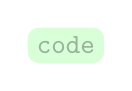
\begin{tikzpicture}
\node[opacity=0.3,fill=green!50,rounded corners,text=black] at (0,0) { \texttt{code} } ;
\end{tikzpicture} 
& Indicates the starting location of the error.\\\\

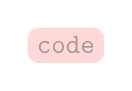
\begin{tikzpicture}
 \node[fill opacity=0.3,fill=red!50,rounded corners] 
    at (0,0) { \texttt{code} };
\end{tikzpicture} & Indicates issues related to the error.\\\\

\begin{tikzpicture}
\draw[>=latex,->] (0,0) -| (1em, 1em );
\end{tikzpicture}  & Arrows can be followed. They indicate the next relevant location to check.\\\\


\begin{tikzpicture}
 \node[circle,draw=gray,very
    thin,fill=black,text=white,inner sep=1pt] at (0,0) {\tiny 1};
\end{tikzpicture} & Enumerations are used to number items of potential interest, especially when the information doesn't fit within the source code.\\\\


\begin{tikzpicture}
\node (node 1) at (0,0) [circle,draw=gray,very
    thin,fill=red!10,text=white,inner sep=1pt,draw=black,text=black] at (0,0) {\tiny \textbf{?}};
\end{tikzpicture} & The compiler expected an associated item, but cannot find it.\\\\


\begin{tikzpicture}
  \node[draw=red,cross out,inner sep=2pt,fill=black,text=white,thick] at (0,0) {};
\end{tikzpicture} & Indicates a conflict between items.\\\\

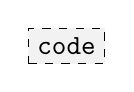
\begin{tikzpicture}
\node[draw,rectangle,draw=black,fill=gray!10,dashed,right] at (0,0) {\texttt{code}};
\end{tikzpicture} & Explanatory code or code generated internally by the compiler. The code is not in the original source.\\\\

\begin{tikzpicture}
\draw (0,0) -- (0,-4em);
\draw[>=square,->,draw=green!50,fill=green!50]    
      (0,-1em) -- +(-3em, 0em);
  \draw[>=square,->,draw=red!50,fill=red!50]
    (0,-2em) -- +(-3em, 0em);
  \draw[>=square,->,draw=green!50,fill=green!50] 
    (0,-3em) -- +(-3em, 0em); -- +(-3em, 0em);
\end{tikzpicture} & Indicates code coverage. Green lines indicate successfully executed code. Red lines indicate failed or skipped lines.\\

\bottomrule
\end{tabularx}
\end{table}
\renewcommand{\tabularxcolumn}[1]{p{#1}}